\documentclass{article}
\usepackage{amsmath, sfmath, multicol, tkz-euclide, array, enumerate, tcolorbox, tabularray}
\renewcommand{\familydefault}{\sfdefault}
\setlength{\parindent}{0cm}
\pagestyle{empty}
\usepackage[left=1in, top=0.5in, right=1in, bottom=0.5in]{geometry}
\tikzset{>=stealth, label style/.append style={font=\footnotesize}}
\tcbset{colback=white}

\newcounter{example}[section]
\newenvironment{example}[1][]{\refstepcounter{example}\par\medskip
   {\color{red}\textbf{Example~\theexample. #1}}}{\medskip}

\begin{document}

\section*{Translations}

\begin{tcolorbox}[colframe=orange!70!white, coltitle=black, title=\textbf{Today I Can}]
\begin{enumerate}
    \item Identify isometries.
    \item Find translation images of figures.
\end{enumerate}
\end{tcolorbox}
\smallskip 

\subsection*{Transformations}

\begin{tcolorbox}[colframe=black!20!white, opacitybacktitle=0.1, coltitle=black, title=\textbf{Transformation}]
A function, or \emph{mapping} that results in a change in the position, shape, or size of a figure.

\begin{itemize}
    \item The \textbf{pre-image} is the original figure (BEFORE)
    \item The \textbf{image} is the resulting figure (AFTER)
\end{itemize}
\end{tcolorbox}

\begin{tcolorbox}[colframe=black!20!white, opacitybacktitle=0.1, coltitle=black, title=\textbf{Rigid Motion}]
A transformation that preserves distance and angle measures (i.e. figures will be congruent).
\end{tcolorbox}

\begin{example}
Does the transformation appear to be a rigid motion?
\begin{multicols}{3}
\begin{enumerate}
    \item \mbox{} \newline 
    
\begin{tikzpicture}[scale=0.3]
    \tkzDefPoints{0/0/A, 1/0/B, 1/1/C, 0/1/D}
    \tkzDrawPolygon(A,B,C,D)
    \tkzLabelSegment[below](A,B){\footnotesize Pre-image}
    \end{tikzpicture}
    \hspace{0.15in}
    
\begin{tikzpicture}[scale=0.8]
    \tkzDefPoints{0/0/A, 1/0/B, 1/1/C, 0/1/D}
    \tkzDrawPolygon(A,B,C,D)
    \tkzLabelSegment[below](A,B){\footnotesize  Image}
    \end{tikzpicture}

    \item \mbox{} \newline 
    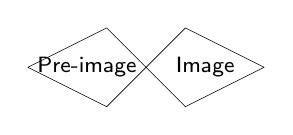
\begin{tikzpicture}[scale=0.5]
    \tkzDefPoints{0/0/A, -1/1/B, -3/0/C, -1/-1/D, 1/1/E, 3/0/F, 1/-1/G}
    \tkzDrawPolygon(A,B,C,D)
    \tkzDrawPolygon(A,E,F,G)
    \node at (-1.5,0) {\footnotesize  Pre-image};
    \node at (1.5,0) {\footnotesize  Image};
    \end{tikzpicture}

    \item \mbox{} \newline 
    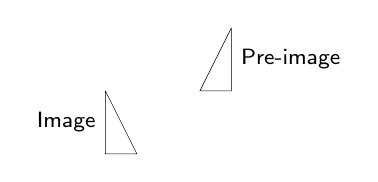
\begin{tikzpicture}[scale=0.4]
    \tkzDefPoints{0/0/A, 1/0/B, 0/2/C}
    \tkzDrawPolygon(A,B,C)
    \tkzLabelSegment[left](A,C){\footnotesize Image}
    \tkzDefShiftPoint[A](4,2){D}
    \tkzDefShiftPoint[B](2,2){E}
    \tkzDefShiftPoint[C](4,2){F}
    \tkzDrawPolygon(D,E,F)
    \tkzLabelSegment[right](D,F){\footnotesize Pre-image}
    \end{tikzpicture}
\end{enumerate}
\end{multicols}
\end{example}

\subsubsection*{Notation}

Transformations can be described using \textbf{arrow notation}. \\
\textbf{Prime notation} is sometimes used to identify image points.

\begin{center}
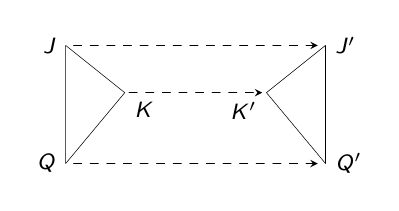
\begin{tikzpicture}[scale=0.6]
\tkzDefPoints{0/0/K, -1.25/1/J, -1.25/-1.5/Q}
\tkzDrawPolygon(K,J,Q)
\tkzLabelPoints[left](J,Q)
\tkzLabelPoints[below right](K)
\tkzDefPoints{3/0/A, 4.25/1/B, 4.25/-1.5/C}
\tkzDrawPolygon(A,B,C)
\tkzLabelPoint[below left](A){$K'$}
\tkzLabelPoint[right](B){$J'$}
\tkzLabelPoint[right](C){$Q'$}
\tkzDrawSegments[->, >=stealth, dashed, add = -0.03 and -0.03](Q,C K,A J,B)
\end{tikzpicture}
\end{center}
\vspace{-0.2in}
\begin{align*}
\triangle JKQ &\rightarrow \triangle J'K'Q' \\
\triangle JKQ &\text{ maps onto } \triangle J'K'Q'
\end{align*}

\begin{example}
In the diagram, $EFGH \rightarrow E'F'G'H'$.
\newline\\

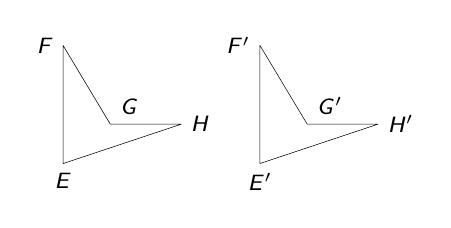
\begin{tikzpicture}
\tkzDefPoints{0/0/E, 0/1.5/F, 1.5/0.5/H, 0.6/0.5/G}
\tkzDrawPolygon(E,F,G,H)
\tkzLabelPoints[right](H)
\tkzLabelPoints[below](E)
\tkzLabelPoints[left](F)
\tkzLabelPoints[above right](G)
\tkzDefShiftPoint[E](0:2.5){E'}
\tkzDefShiftPoint[F](0:2.5){F'}
\tkzDefShiftPoint[G](0:2.5){G'}
\tkzDefShiftPoint[H](0:2.5){H'}
\tkzDrawPolygon(E',F',G',H')
\tkzLabelPoints[right](H')
\tkzLabelPoints[below](E')
\tkzLabelPoints[left](F')
\tkzLabelPoints[above right](G')
\end{tikzpicture}

\begin{multicols}{2}
\begin{enumerate}[(a)]
\item What are the images of $\angle F$ and $\angle H$?
\item What are the pairs of corresponding sides?
\end{enumerate}
\end{multicols}
\end{example}

\newpage 

\subsection*{Translations}

\begin{tcolorbox}[colframe=black!20!white, opacitybacktitle=0.1, coltitle=black, title=\textbf{Translation}]
A transformation that maps all points of a figure the same distance in the same direction (i.e. a \emph{slide} of the original figure).

\begin{minipage}{0.6\textwidth}
\begin{itemize}
    \item Corresponding parts (angles and sides) will be congruent.
    \item Every point gets moved according to the rule.
\end{itemize}
\end{minipage}
\begin{minipage}{0.3\textwidth}
    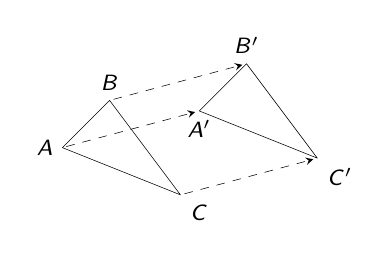
\begin{tikzpicture}[scale=0.6]
    \tkzDefPoints{0/0/A, 1/1/B, 2.5/-1/C}
    \tkzLabelPoints[left](A)
    \tkzLabelPoints[above](B)
    \tkzLabelPoints[below right](C)
    \tkzDrawPolygon(A,B,C)
    \tkzDefShiftPoint[A](15:3){A'}
    \tkzDefShiftPoint[B](15:3){B'}
    \tkzDefShiftPoint[C](15:3){C'}
    \tkzDrawPolygon(A',B',C')
    \tkzLabelPoints[below](A')
    \tkzLabelPoints[above](B')
    \tkzLabelPoints[below right](C')
    \tkzDrawSegments[->, >=stealth, dashed, add = -0.03 and -0.03](A,A' B,B' C,C')
    \end{tikzpicture}
\end{minipage}
\end{tcolorbox}
\smallskip 

\begin{example}
Graph each of the following. Write the coordinates of the translated image.
\begin{multicols}{2}
\begin{enumerate}[(a)]
    \item $T(3, \, 5), \, C(4, \, 5), \, Z(4, \, 4)$ \\ translate 6 units left and 3 units down.
    \item $A(3, \, -1), \, L(3, \, -5), \, U(1, \, -5), \, K(1, \, -2)$ \\ translate 3 units right and 4 units up.
\end{enumerate}
\end{multicols}
\begin{tabular}{p{0.5\textwidth}p{0.5\textwidth}}
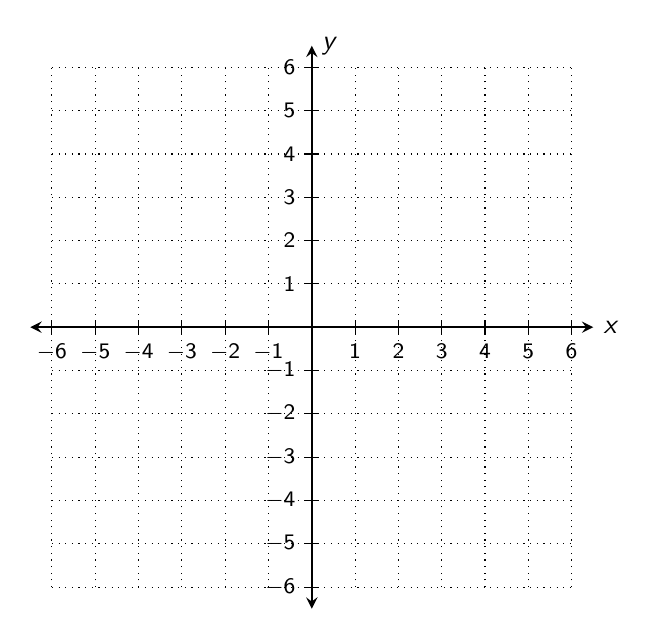
\begin{tikzpicture}[scale=0.55]
\draw[<->, thick] (-6.5,0) -- (6.5,0) node [right] {$x$};
\draw[<->, thick] (0,-6.5) -- (0,6.5) node [right] {$y$};
\draw[dotted] (-6,-6) grid (6,6);
\foreach \x in {-6,...,-1,,1,...,6}
\draw (\x, 0.15) -- (\x,-0.15) node [below] {\footnotesize $\x$};
\foreach \y in {-6,...,-1,,1,...,6}
\draw (0.15,\y) -- (-0.15,\y) node [left] {\footnotesize $\y$};
\end{tikzpicture}
&
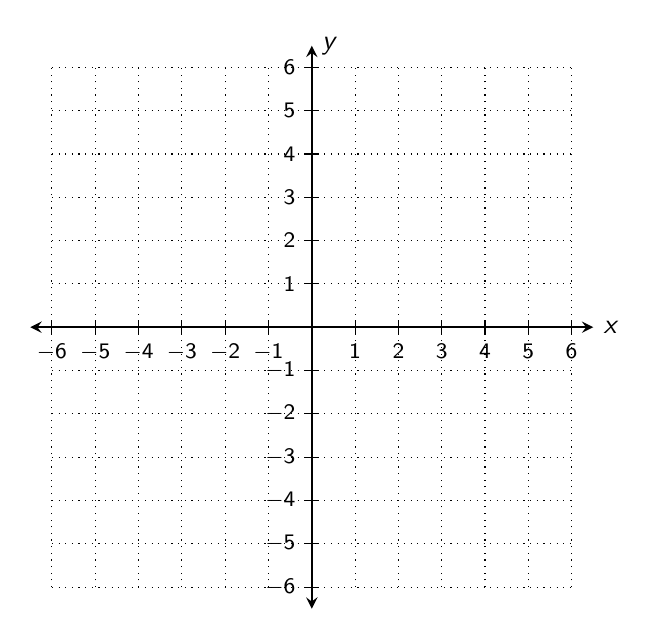
\begin{tikzpicture}[scale=0.55]
\draw[<->, thick] (-6.5,0) -- (6.5,0) node [right] {$x$};
\draw[<->, thick] (0,-6.5) -- (0,6.5) node [right] {$y$};
\draw[dotted] (-6,-6) grid (6,6);
\foreach \x in {-6,...,-1,,1,...,6}
\draw (\x, 0.15) -- (\x,-0.15) node [below] {\footnotesize $\x$};
\foreach \y in {-6,...,-1,,1,...,6}
\draw (0.15,\y) -- (-0.15,\y) node [left] {\footnotesize $\y$};
\end{tikzpicture}
\end{tabular}
\end{example}

\vfill 

\begin{example}
Write the rule for the given translation.
\newline\\

\begin{tabular}{p{0.5\textwidth}p{0.5\textwidth}}
(a) &   (b)     \\[0.1in]
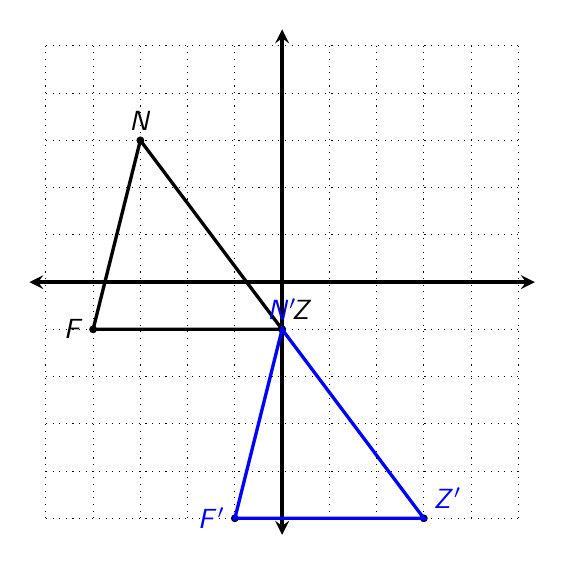
\begin{tikzpicture}[scale=0.6]
\draw [<->, >=stealth, very thick] (-5.35,0) -- (5.35,0);
\draw [<->, >=stealth, very thick] (0,-5.35) -- (0,5.35);
\draw [dotted] (-5,-5) grid (5,5);
\coordinate (N) at (-3,3);
\coordinate (F) at (-4,-1);
\coordinate (Z) at (0,-1);
\draw [fill=black] (N) circle (2pt);
\draw [fill=black] (F) circle (2pt);
\draw [fill=black] (Z) circle (2pt);
\draw [very thick] (N) -- (F) -- (Z) -- cycle;
\node at (F) [anchor = east] {$F$};
\node at (N) [anchor = south] {$N$};
\node at (Z) [anchor = south west] {$Z$};
\coordinate (N') at (0,-1);
\coordinate (F') at (-1,-5);
\coordinate (Z') at (3,-5);
\draw [fill=blue] (N') circle (2pt);
\draw [fill=blue] (F') circle (2pt);
\draw [fill=blue] (Z') circle (2pt);
\draw [very thick, blue] (N') -- (F') -- (Z') -- cycle;
\node at (F') [anchor = east, color=blue] {$F'$};
\node at (N') [anchor = south, color=blue] {$N'$};
\node at (Z') [anchor = south west, color=blue] {$Z'$};
\end{tikzpicture}
&
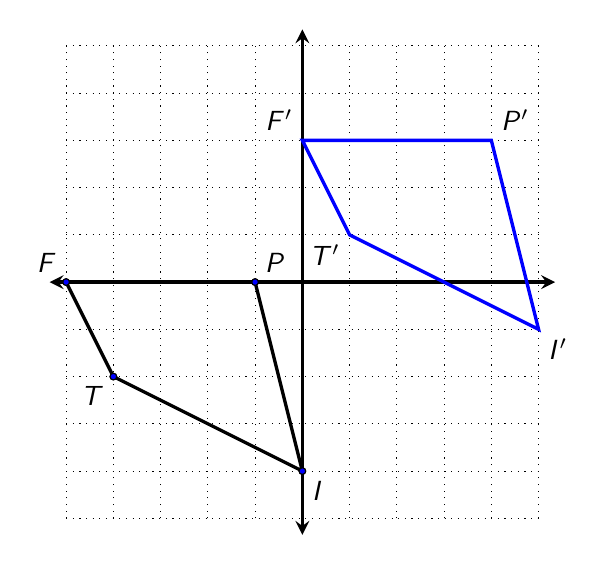
\begin{tikzpicture}[scale=0.6]
\draw [<->, >=stealth, very thick] (-5.35,0) -- (5.35,0);
\draw [<->, >=stealth, very thick] (0,-5.35) -- (0,5.35);
\draw [dotted] (-5,-5) grid (5,5);
\coordinate (F) at (-5,0);
\coordinate (T) at (-4,-2);
\coordinate (I) at (0,-4);
\coordinate (P) at (-1,0);
\draw [fill=black] (F) circle (2pt);
\draw [fill=black] (T) circle (2pt);
\draw [fill=black] (I) circle (2pt);
\draw [fill=black] (P) circle (2pt);
\draw [very thick] (F) -- (T) -- (I) -- (P);
\node at (F) [anchor = south east] {$F$};
\node at (T) [anchor = north east] {$T$};
\node at (I) [anchor = north west] {$I$};
\node at (P) [anchor = south west] {$P$};
\coordinate (F') at (0,3);
\coordinate (T') at (1,1);
\coordinate (I') at (5,-1);
\coordinate (P') at (4,3);
\draw [fill=blue] (F) circle (2pt);
\draw [fill=blue] (T) circle (2pt);
\draw [fill=blue] (I) circle (2pt);
\draw [fill=blue] (P) circle (2pt);
\draw [very thick, color=blue] (F') -- (T') -- (I') -- (P') -- cycle;
\node at (F') [anchor = south east] {$F'$};
\node at (T') [anchor = north east] {$T'$};
\node at (I') [anchor = north west] {$I'$};
\node at (P') [anchor = south west] {$P'$};
\end{tikzpicture}
\end{tabular}
\end{example}

\end{document}
